\scanpage{19}
% archive sheet number: 18

Plus généralement, on a

\[
\begin{aligned}
\overline{Z^*_A}&=Z^*_{\overline A}\\
\left(\ \bigcup_{\alpha\in A}\overset{\shortparallel}{\overline{Z_\alpha}}=\bigcup_{\deleted{\unsure{\beta}}\alpha\in A}Z_{\overline{\{\alpha\}}}
=Z_{\underbrace{\bigcup_{\alpha\in A}\overline{\{\alpha\}}}_{\overline A}}\ \right)&
\end{aligned}
\]

L'ens \deleted{$\Sigma$} ordonné $\Sigma$ est \deleted{donc un} \inserted{donc} l'ens d'indices d'une stratification \inserted{(finie)} de la sphère $S$, satisfaisant l'axiome de fidélité \inserted{et de} densité \deleted{(toute cellule \deleted{ouverte} $Z_\alpha$ est dense} (les $Z^*_\alpha\ne\varnothing$, $\overline{Z^*_\alpha}=Z_\alpha$)\deleted{\unsure{et}} , et à strates \unsure{connexes|convexes}.

\deleted{$\Sigma$ en général n'est pas \deleted{un Inf} \inserted{un ens} réticulé i.e. deux éléments de $\Sigma$ qui sont minorés n'ont pas néc$^{\mathrm{t}}$. de $\operatorname{Inf}$ -- ex. $V$ de dim $3$, avec $n\geq\unsure{2|1|3}$ plans passant par une $=$ droite (p.ex. $n=2$). Mais \unsure{sauf erreur|sans aucune|sans doute}, si l'intersection des $H_i$ est réduite à $\{0\}$, alors l'intersection de deux \deleted{\unsure{pla}} facettes fermées est une facette fermée.}

\margin{?}

\figure{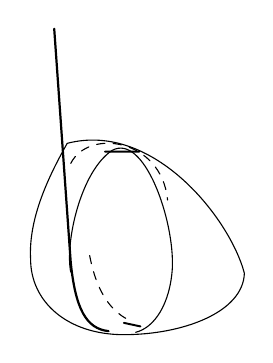
\begin{tikzpicture}[x=0.015cm,y=-0.015cm,line cap=round,line join=round,inner sep=0.4pt]
\draw (46,30)..controls(119,11)and(184,94)..(196,140)..controls(195,173)and(144,192)..(94,192)..controls(46,192)and(15,164)..(15,128)..controls(13,92)and(32,55)..(46,30);
\draw[thick] (35,-67)--(49,131)..controls(53,170)and(62,187)..(81,189);
\draw (49,139)..controls(44,115)and(57,54)..(84,36)..controls(111,21)and(137,95)..(135,136)..controls(133,166)and(120,186)..(104,190);
\draw[dashed] (49,47)..controls(64,17)and(126,26)..(131,78) (65,125)..controls(70,151)and(80,171)..(99,180);
\draw[line width=.7pt] (78,37)--(107,37) (94,182)--(108,185);

\end{tikzpicture}}

$\Sigma$ est une partie ouverte de $E$ i.e. $\alpha\in\Sigma$, $\beta\in E$, $\beta>\alpha$ implique $\beta\in\Sigma$. Donc dans $\Sigma$ comme dans $E$, tte partie majorée a un Sup (car c'est le cas \deleted{dans} $\mathbb F_3$) \inserted{de m} \deleted{\unsure{tout|toute}} partie minorée de $\Sigma$ a un Inf.
